\documentclass[14pt,oneside]{extarticle}

\usepackage{amsmath}
\usepackage{unicode-math}
\renewcommand{\familydefault}{\rmdefault}
\usepackage{mathtext}
\usepackage{geometry}
\geometry{verbose,lmargin=25mm,rmargin=15mm,tmargin=15mm,bmargin=20mm}
\setcounter{secnumdepth}{3}
\setcounter{tocdepth}{3}
\usepackage{setspace}
\setstretch{1.5}

% Картинки (можно встявлять даже pdf)
\usepackage{graphicx}

% Таблицы
\usepackage{tabularx}
% \setlength{\extrarowheight}{0.3cm}
\renewcommand{\arraystretch}{1.5}
\renewcommand{\tabularxcolumn}[1]{>{\centering\arraybackslash\small}m{#1}}
\newcolumntype{B}{>{\bfseries\small}c}
\newcolumntype{R}{>{\small}c}
%% Because html converters don't know tabularnewline
\providecommand{\tabularnewline}{\\}

\makeatletter
%%%%%%%%%%%%%%%%%%%%%%%%%%%%%% Textclass specific LaTeX commands.
\numberwithin{figure}{section}
\numberwithin{table}{section}
\numberwithin{equation}{section}
\makeatother

% Абзацный отступ = 1.25см
\usepackage{indentfirst}
\setlength\parindent{12.5mm}

% Пакет для содержания
\usepackage{tocloft}

% Команда для специальных разделов (введение, обзор литературы, etc)
% Не нумеруются в содержании, по уровню вложенности: 
\newcommand{\specialsection}[1]{
    \phantomsection
    \bigskip\smallskip\hspace{-13.8mm}
    \normalfont\fontsize{18}{18}\textbf{#1}
    \par\bigskip\normalfont\normalsize
    \addcontentsline{toc}{section}{#1}
}

% Размеры заголовков разделов и подразделов
\usepackage{titlesec}
% Раздел: 18pt, добавляем слово "Глава"
\titleformat{\section}
{\fontsize{18}{18}\bfseries}{
\hspace{-1.5mm}Глава \thesection. \hskip-1em}{1em}{}
% Подраздел: 16pt
\titleformat{\subsection}
{\fontsize{16}{16}\bfseries}{\hspace{-0.2mm}\thesubsection}{1em}{}

% Содержание
% Выравнивание заголовка по центру (да, да, с отступом слева)
% т.к. окружение center и \centering не работают
\renewcommand{\cfttoctitlefont}{\hspace{0.35\textwidth} \bfseries\Large}
% \renewcommand{\cftbeforetoctitleskip}{3em}
% Слово "Глава" в содержании
\renewcommand{\cftsecpresnum}{Глава\space}
\newlength\mylength
\settowidth\mylength{\cftsecpresnum}
\addtolength\cftsecnumwidth{1.5\mylength}
% Строки с точками
\renewcommand{\cftsecleader}{\cftdotfill{\cftdotsep}}
% Точки после цифр в в содержании
\renewcommand{\cftsecaftersnum}{.}
\renewcommand{\cftsubsecaftersnum}{.}
% Подровнять subsection под точку главы
% (если глав будет больше десяти, будет чуть хуже)
\setlength{\cftsubsecindent}{2em}
% Интервал глав
\setlength{\cftbeforesecskip}{3pt}

\renewcommand{\cftsecpagefont}{\normalfont}

\usepackage[russian]{babel}
\usepackage{fontspec}
\setmainfont{Times New Roman}
\setmathfont{TeX Gyre Termes Math}
\usepackage{csquotes}

% Пакет, реализующий гиперссылки. Никакого расскрашивания
\usepackage[colorlinks=false,unicode=true,hidelinks]{hyperref}

\newcommand{\ITEM}{\vspace{-0.2cm}\item}
\newcommand{\MList}[1]{\par\begin{itemize}#1\end{itemize}}
\newcommand{\NList}[1]{\par\begin{enumerate}#1\end{enumerate}}

% Шрифт подписи (caption) = 12pt
% (Повезло, что small как раз равен 12pt)
\usepackage[font=small,labelfont=bf]{caption}

% Пакет, который позволяет собирать один документ TeX из нескольких
\usepackage{import}

%Библиография
\usepackage[
    backend=biber,
    %citestyle = alphabetic, 
    %bibstyle = ieee-alphabetic,  
    %sortlocale=en_US,
    sorting=none,
    backref=true,
    hyperref=true,
    style=numeric,%style=alphabetic,
    defernumbers=true,
    isbn=false,
    autolang=none,
    %eid=true,
    doi=false,
    %series=true,
    eprint=false,
    bibencoding = utf8
]{biblatex} %Imports biblatex package

\renewbibmacro{volume+number+eid}{%
    \printfield{volume}%
    \setunit{\addcomma\space}%
    \printfield{number}%
    \printfield{eid}}

\renewbibmacro{in:}{\space}

\DeclareFieldFormat[article]{volume}{{том}\space#1}
\DeclareFieldFormat[article]{number}{{номер}\space#1\addcomma}

\DefineBibliographyStrings{russian}{%
    phdthesis = {диссертация}%
}

\addbibresource{literature.bib} %Import the bibliography file

% Подсветка кода (все стили в файле)
\usepackage{color}
\usepackage{listings}
\definecolor{GrayCodeBlock}{RGB}{248,252,255}
\definecolor{BlackText}{RGB}{41,75,102}
\definecolor{RedTypename}{RGB}{182,86,17}
\definecolor{GreenString}{RGB}{96,172,57}
\definecolor{PurpleKeyword}{RGB}{184,84,212}
\definecolor{GrayComment}{RGB}{100,100,100}
\definecolor{GoldDocumentation}{RGB}{180,165,45}

\lstset{
    columns=fullflexible,
    keepspaces=true,
    frame=single,
    framesep=0pt,
    framerule=0pt,
    framexleftmargin=4pt,
    framexrightmargin=4pt,
    framextopmargin=5pt,
    framexbottommargin=3pt,
    xleftmargin=4pt,
    xrightmargin=4pt,
    backgroundcolor=\color{GrayCodeBlock},
    basicstyle=\ttfamily\small\color{BlackText},
    keywordstyle=\color{PurpleKeyword},
    ndkeywordstyle=\color{RedTypename},
    comment=[l][\color{GrayComment}\slshape]{//},
    morecomment=[s][\color{GrayComment}\slshape]{/*}{*/},
    morecomment=[s][\color{RedTypename}]{\#![}{]},
    morecomment=[s][\color{RedTypename}]{\#[}{]},
    stringstyle=\color{GreenString},
    string=[b]"
}

\lstdefinelanguage{rust}
{
    keywords={
        true,false,
        unsafe,async,await,move,
        use,pub,crate,super,self,mod,
        struct,enum,fn,const,static,let,mut,ref,type,impl,dyn,trait,where,as,
        break,continue,if,else,while,for,loop,match,return,yield,in
    },
    ndkeywords={
        bool,u8,u16,u32,u64,u128,i8,i16,i32,i64,i128,char,str,
        Self,Option,Some,None,Result,Ok,Err,String,Box,Vec,Rc,Arc,Cell,RefCell,HashMap,BTreeMap,
        macro_rules
    },
    comment=[l][\color{GrayComment}\slshape]{//}
}


\begin{document}

\newgeometry{left=30mm, top=20mm, right=15mm, bottom=20mm, nohead, nofoot}
\begin{titlepage}
\begin{center}
Министерство высшего образования и науки Российской федерации

Федеральное государственное автономное \\образовательное учреждение высшего образования

\textbf{<<Национальный исследовательский ядерный университет}
\textbf{<<МИФИ>>}

\vspace{25mm}

\textbf{\textit{\large Фамилия Имя Отчество}} \\[8mm]
% Название
\textbf{\large Выпускная квалификационная работа}\\[3mm]
\textbf{\textit{\large Название работы}}

\vspace{10mm}
Уровень образования: бакалавриат / магистратура\\
Направление 11.04.04 «Электроника и наноэлектроника»\\
Образовательная программа
«Наноэлектроника, спинтроника и фотоника»

\vspace{15mm}

% Научный руководитель, рецензент
\begin{flushleft}
\textbf{Выпускник:} Фамилия И.О.

\hspace{10cm} \textit{Подпись}: \space \hrulefill

\textbf{Научный руководитель:} 

к.ф.-м.н., доцент кафедры физики конденсированных сред

ИНТЭЛ НИЯУ МИФИ, Фамилия И.О.

\hspace{10cm} \textit{Подпись}: \space \hrulefill

\textbf{И.о. заместителя заведующего кафедрой:} 

д.ф.-м.н., профессор кафедры физики конденсированных сред 

ИНТЭЛ НИЯУ МИФИ, Никитенко В.Р.

\hspace{10cm} \textit{Подпись}: \space \hrulefill \space
\end{flushleft}

\vfill 

{Москва}
\par{\the\year{} г.}
\end{center}
\end{titlepage}
% Возвращаем настройки geometry обратно (то, что объявлено в преамбуле)
\restoregeometry
% Добавляем 1 к счетчику страниц ПОСЛЕ titlepage, чтобы исключить 
% влияние titlepage environment
\addtocounter{page}{1}


% Содержание
\tableofcontents
\pagebreak

% ============================================
% ВВЕДЕНИЕ
% ============================================
\specialsection{Введение}

Здесь необходимо рассказать, о чём работа. Объём 1-2 страницы. Нужно охарактеризовать область исследования, практическую значимость (для разработки каких приборов могут быть использованы ваши результаты), какую проблему решает ваша работа (кратко, подробнее будет в обзоре), какие методы использованы (тоже кратко, подробнее в главе Методы).

Здесь необходимо рассказать, о чём работа. Объём 1-2 страницы. Нужно охарактеризовать область исследования, практическую значимость (для разработки каких приборов могут быть использованы ваши результаты), какую проблему решает ваша работа (кратко, подробнее будет в обзоре), какие методы использованы (тоже кратко, подробнее в главе Методы).

Здесь необходимо рассказать, о чём работа. Объём 1-2 страницы. Нужно охарактеризовать область исследования, практическую значимость (для разработки каких приборов могут быть использованы ваши результаты), какую проблему решает ваша работа (кратко, подробнее будет в обзоре), какие методы использованы (тоже кратко, подробнее в главе Методы).

\specialsection{Цель и задачи}
\label{Tasks}

\textbf{Цель:} Цель не должна совпадать с темой работы. Цель должна быть достижима (должен быть конечный результат) и проверяема. Исследование --- это процесс, и целью быть не может.

\textbf{Задачи}
\begin{enumerate}
    \item Задача 1
    \item Задача 2
    \item Задача 3
    \item Задача 4
\end{enumerate}

Достаточно задач. Обзор литературы наверное в задачи включать не будем. Лучше написать конкретно, что мы делаем (разработка алгоритма, программная реализация, расчёт конкретных параметров при определённых условиях и т.д.)

% ============================================
% ГЛАВА 1
% ============================================
\pagebreak
\section{Обзор литературы}

\subsection{Раздел 1}

В обзоре не нужно рассказывать теорию и методы, нужно просто провести обобщение и анализ исследований, которые были проведены до вас по данной теме.

Если вы будете пользоваться какими-то терминами и понятиями, которые требуют разъяснения, их нужно объяснить в следующих двух главах, а отсюда можно сослаться на эти определения.

Ссылка на книгу: \cite{datta1}.
Ссылка на книгу на русском: \cite{fedotkin1}.

\begin{figure}[ht]
\begin{center}
    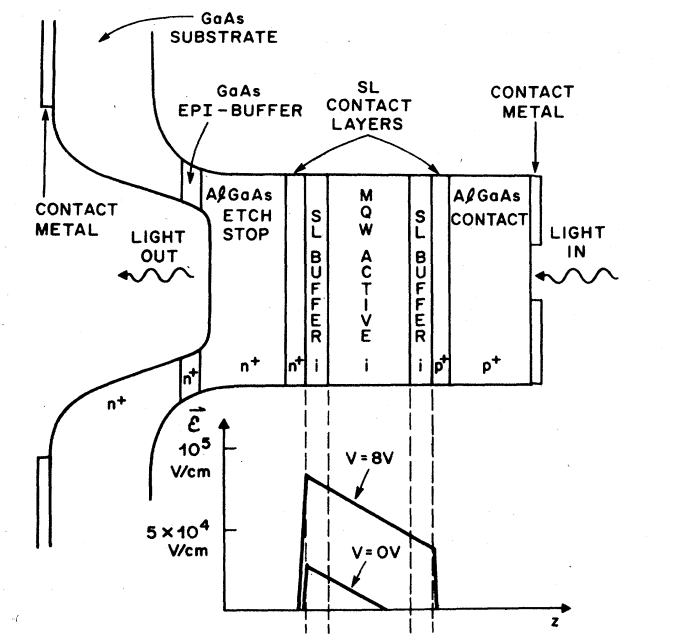
\includegraphics[width=11cm]{images/Miller2-Figure2.png}
    \caption{\label{fig:miller2-2}
        Схема измерений спектров поглощения в поперечном поле из работы \cite{miller1}.}
\end {center}
\end {figure}
    
Если рисунок взят из какой-то статьи, книги или из интернета (из интернета нежелательно), то нужно обязательно в подписи сделать ссылку на соответствующий пункт в списке литературы.

Ссылаемся на рисунок \ref{fig:miller2-2}.

Рисунки в формате pdf:

\begin{figure}[ht]
    \begin{center}
        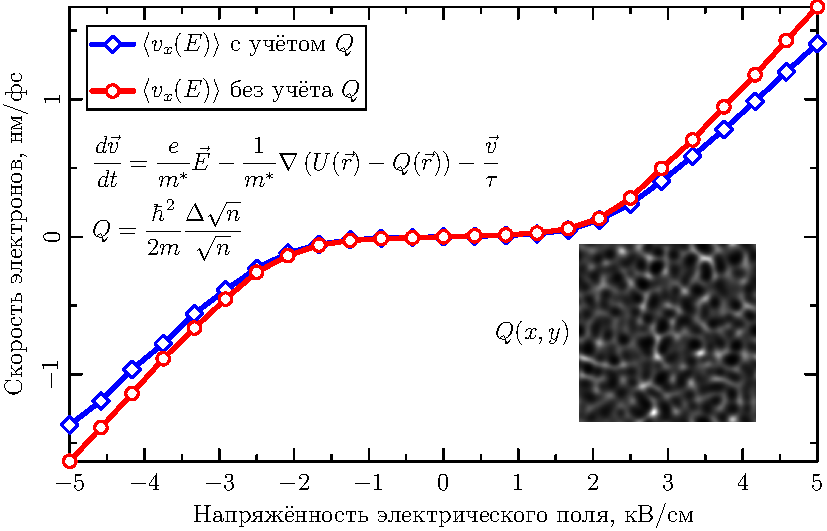
\includegraphics{images/iv-curve.pdf}
        \caption{\label{fig:iv-curve-1}
            Результаты моделирования траекторий электронов с помощью квантовых гидродинамических уравнений.}
    \end {center}
\end {figure}

\begin{figure}[ht]
    \begin{center}
        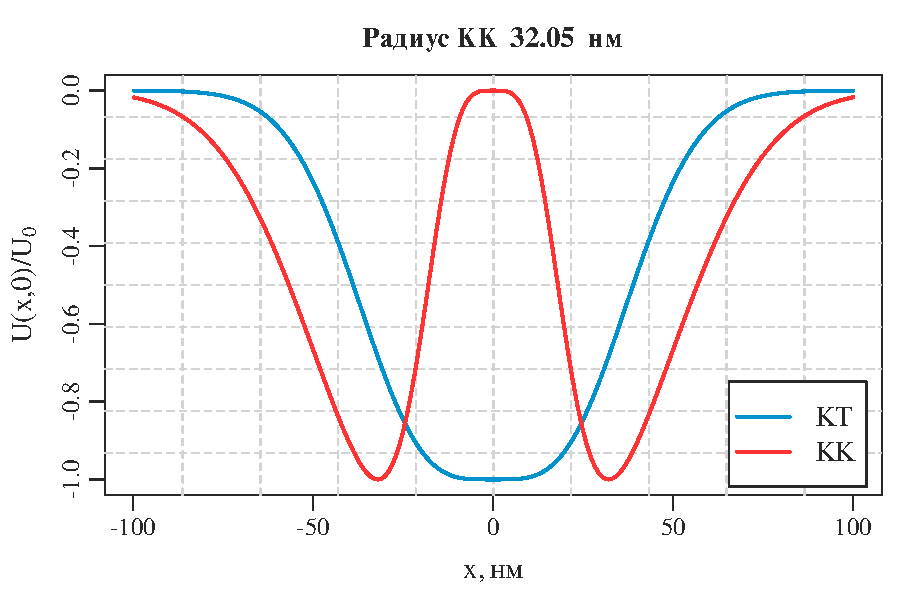
\includegraphics{images/qd_qr_potential.pdf}
        \caption{\label{fig:qr-potential-1}
            Потенциалы для моделирования КТ и КК.}
    \end {center}
\end {figure}
    
Ссылки на статьи: \cite{miller1}, \cite{miller2}, \cite{mohseni1}.

Ссылка на российскую статью: \cite{skubachevskii1}.

Ссылка на диссертацию:  \cite{pavlichenko1}

% ============================================
% ГЛАВА 2
% ============================================
\pagebreak
\section{Теория и основные уравнения}

\subsection{Раздел 1}

Ненумерованная формула:

\begin{equation}
    \begin{pmatrix} \dot{\varphi}\\ \dot{\theta} \\ \dot{\psi} \end{pmatrix}
    = \begin{pmatrix}
        \cos(\theta)\cos(\psi) & -\sin(\psi) & 0 \\
        \cos(\theta)\sin(\psi) & \cos(\psi)  & 0 \\
        -\sin(\theta)         & 0         &  1
    \end{pmatrix}^{-1}
    \begin{pmatrix} \omega_x\\ \omega_y \\ \omega_z \end{pmatrix}. \nonumber
\end{equation}


\begin{equation}
    E_{y}\left(z\geq L\right)=A_{12}e^{i\beta z}\cdot\begin{cases}
        e^{sw}\cos\left(kw\right)e^{s\left(x-a\right)}, & x<a-w\\
        \cos\left(k\left(x-a\right)\right), & a-w\leq x\le a+w\\
        e^{sw}\cos\left(kw\right)e^{-s\left(x-a\right)}, & x>a+w
        \end{cases}    
\end{equation}


\subsection{Раздел 2}

Нумерованные формулы:

\begin{equation}
\label{eq:1}
    \dot{\theta}=\frac{P-p_{1}\cos\left(\varphi_{1}-\theta\right)-p_{2}\cos\left(\varphi_{2}-\theta\right)}{\mu+\sin^{2}\left(\varphi_{1}-\theta\right)+\sin^{2}\left(\varphi_{2}-\theta\right)}
\end{equation}

\begin{equation}
    \dot{\varphi}_{1}=p_{1}-\dot{\theta}\cos(\phi_{1}-\theta)
\end{equation}

\begin{equation}
    \dot{\varphi}_{2}=p_{2}-\dot{\theta}\cos(\phi_{2}-\theta)
\end{equation}

Тест ссылки на формулу (\ref{eq:1}).

% ============================================
% ГЛАВА 3
% ============================================
\pagebreak
\section{Численные методы и алгоритмы}

\subsection{Раздел 1}

\subsection{Раздел 2}

% ============================================
% ГЛАВА 4
% ============================================
\pagebreak
\section{Программная реализация}

\begin{lstlisting}[language=rust,caption={Программная реализация метода Рунге-Кутты},label={listing-1}]
    // From the pendulum program
    fn runge_kutta(
        vars: &MyVec,
        pars: &Vec<f64>,
        rhs: &dyn Fn(&MyVec, &Vec<f64>) -> MyVec,
        dt: f64,
    ) -> MyVec {
        let rk_1 = rhs(vars, pars);
        let rk_2 = rhs(&vars.add(&rk_1.scale(dt / 2.0)), pars);
        let rk_3 = rhs(&vars.add(&rk_2.scale(dt / 2.0)), pars);
        let rk_4 = rhs(&vars.add(&rk_3.scale(dt)), pars);
    
        let vars_new = vars
            .add(&rk_1.scale(dt / 6.0))
            .add(&rk_2.scale(dt / 3.0))
            .add(&rk_3.scale(dt / 3.0))
            .add(&rk_4.scale(dt / 6.0));
        vars_new
    }
    \end{lstlisting}
    
    \begin{lstlisting}[language=C++,caption={Подпрограмма случайного блуждания на плоскости},label={listing-2}]
    std::random_device rd;
    std::mt19937 mt(rd());
    std::uniform_int_distribution<long> dist(1, 4);
    std::vector<long> xn(n0, 0);
    std::vector<long> yn(n0, 0);
    for (long jt = 0; jt < M; jt++)
    {
        for (long jn = 0; jn < n0; jn++)
        {
            switch (dist(mt))
            {
            case 1:
                xn[jn] ++;
                break;
            case 2:
                xn[jn] --;
                break;
            case 3:
                yn[jn] ++;
                break;
            case 4:
                yn[jn] --;
                break;
            }
        }
    }
    \end{lstlisting}

% ============================================
% ГЛАВА 5
% ============================================
\pagebreak
\section{Результаты и обсуждение}

Таблицы в \LaTeX ~делать очень неудобно. Лучше воспользоваться сторонним редактором таблиц, которые умеет их экспортировать в \LaTeX, сделать там всю структуру, а потом вставить готовый код, и в нём уже добавлять содержимое ячеек.

Тем не менее, простые таблицы делать можно, наподобие \ref{table-1}. Но лучше таблицами вообще не злоупотреблять, а где можно заменять их графиками и диаграммами.

\begin{center}
\begin{table}[h]
\centering{}%
\caption{Условия роста образцов с квантовыми кольцами\label{table-1}}
\begin{tabularx}{0.9\textwidth}{|B|R|R|R|R|R|X|X|}
\hline 
№ & $X_{\text{In}}$, \% & $T_1$, °C & $T_2$, °C & $P_{\text{As}_4}$, $10^{-5}$ Торр & Тип КК & \multicolumn{2}{R|}{Диаметры, нм} \tabularnewline
\hline
А1 & 0 & 220 & 220 & 1,3 & Одиночное & \multicolumn{2}{R|}{51} \tabularnewline
\hline
А2 & 0 & 280 & 280 & 0,55 & Двойное & 120 & 42 \tabularnewline
\hline
Б1 & 5 & 250 & 250 & 5,0 & Одиночное & \multicolumn{2}{R|}{75}  \tabularnewline
\hline 
Б2 & 10 & 250 & 250 & 5,0 & Одиночное & \multicolumn{2}{R|}{76}  \tabularnewline
\hline 
Б3 & 20 & 250 & 250 & 5,0 & Одиночное & \multicolumn{2}{R|}{78}  \tabularnewline
\hline 
Б4 & 20 & 200 & 200 & 5,0 & Одиночное & \multicolumn{2}{R|}{63}  \tabularnewline
\hline 
В1 & 0 & 325 & 325 & 0,2 & Одиночное & \multicolumn{2}{R|}{22}  \tabularnewline
\hline 
В2 & 0 & 325 & 220 & 0,2 & Двойное & 79 & 31 \tabularnewline
\hline 
В3 & 0 & 325 & 325 & 1,0 & Двойное & 69 & 27 \tabularnewline
\hline
\end{tabularx}
\end{table}
\end{center}

Ссылаемся на Листинг \ref{listing-1} здесь.

% ============================================
%  ВЫВОДЫ И ЗАКЛЮЧЕНИЕ
% ============================================
\pagebreak
\specialsection{Выводы}
Структура файлов, которые можно редактировать:

\begin{itemize}
    \item \verb|diploma.tex| --- содержит основной текст;
    \item \verb|titlepage.tex| --- содержит титульный лист;
    \item \verb|literature.bib| --- содержит источники для списка литературы;
    \item \verb|code_highlight.tex| --- форматирование листингов (фрагментов кода).
\end{itemize}

Файл \verb|style.tex| очень важный, его трогать и особенно удалять не надо, там задаются различные стили документа. Редактировать в случае, если знаете, что делать.

\specialsection{Заключение}

Нужны ли отдельно и выводы, и заключение --- я не знаю. Разберёмся.

Список литературы ниже оформлен не совсем по ГОСТу, но это легко исправить. Главное, что он организован, и можно ссылаться на каждый пункт по фамилии первого автора.

\textbf{Внимание!} 

Список литературы находится в отдельном файле \verb|literature.bib|, в который можно добавлять новые источники в любом порядке. Они будут сами располагаться как нужно, в порядке упоминания в тексте.

Если какой-то источник не процитирован в тексте, он в список литературы добавлен не будет.

Поэтому один и тот же файл с источниками можно использовать для нескольких документов.


\pagebreak
\printbibliography

\end{document}
